\section{Logical Agent}
	\subsection{Knowledge Based Agents}
		On peut raisoner avec de la connaissance pour savoir quelle action faire. Il y a 2 types de connaissances :
		\begin{enumerate}
			\item \textbf{Logique classique} : Vrai ou fausse
			\item \textbf{Autre logique} : connaissance incertaine
		\end{enumerate}
		
		L'agent peut etre représenté de la sorte : 
		\begin{figure}[htp]
			\centering
			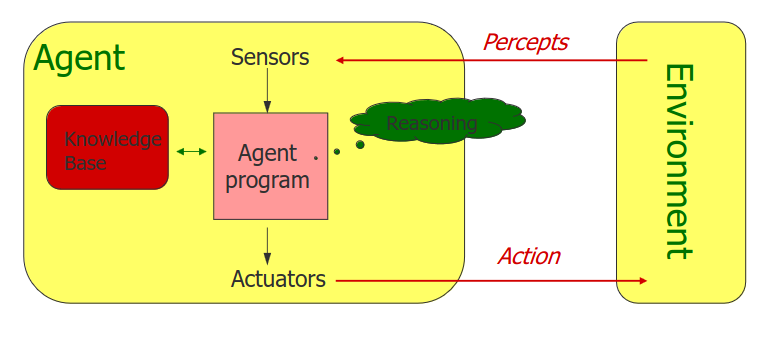
\includegraphics[width=\textwidth]{img/KBA.png}
		\end{figure}
		
		
		Le composant central d'un KBA est un ensemble de phrase (KB).
		
		\textbf{Sentences} : phrase qui est une affirmations sur le monde
			
			
		\subsubsection{Operation KBA}
			\begin{enumerate}
				\item \textbf{TELL :} Ajoute une nouvelle phrase
				\item \textbf{ASK :} Demande se qui est connue
				\item \textbf{MAKE-PERCEPT-SENTENCE} : Construit une phrase affirmant que l'agent a perçu le percept donné à un moment donné.
				\item \textbf{MAKE-ACTION-QUERY} : Construit une phrase qui ASK quelle action devrait etres faite maintenant
				\item \textbf{MAKE-ACTION-SENTENCE} : Construit une phrase affirmant que l'action choisie a été exécutée
			\end{enumerate}
			
			\begin{figure}[htp]
				\centering
				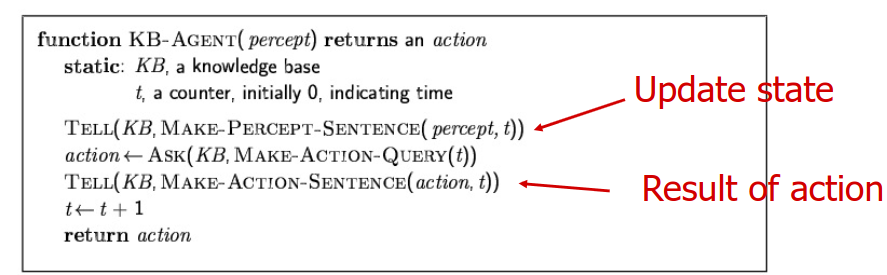
\includegraphics[width=\textwidth]{img/KBA1.png}
			\end{figure}
			
		\subsubsection{Knowledge representation}
			Le language dans laquelle la phrase est représenté. Il y a 2 approches
			\begin{itemize}
				\item \textbf{Declarative approach} : Nous ne disons à l'agent que ce qu'il a besoin de savoir. Les phrases sont dites une à une (par TELL) jusqu'à ce que l'agent sache comment opérer dans son environnement.
				\item \textbf{Procedural approach} : Nous codons les comportements souhaités directement sous forme de programme.
			\end{itemize}
			
	\subsection{Exemple : the Wumpus World}
	
		Une grille avec un créature qui mange les agents. Il y a des puits dans des cases (a éviter) et le but est de trouver le trésor sans se faire manger ni tomber dans les puits.\footnote{pages 209-210-211 du livre}
		\begin{itemize}
			\item Pas entièrement observable (perception local)
			\item Déterministe
			\item Pas épisodique (séquentielle au niveau des actions préformées)
			\item Statique (Monstre et puits ne bouge pas)
			\item Discret
			\item Un seul agent
		\end{itemize}
		
		\begin{figure}[H]
			\centering
			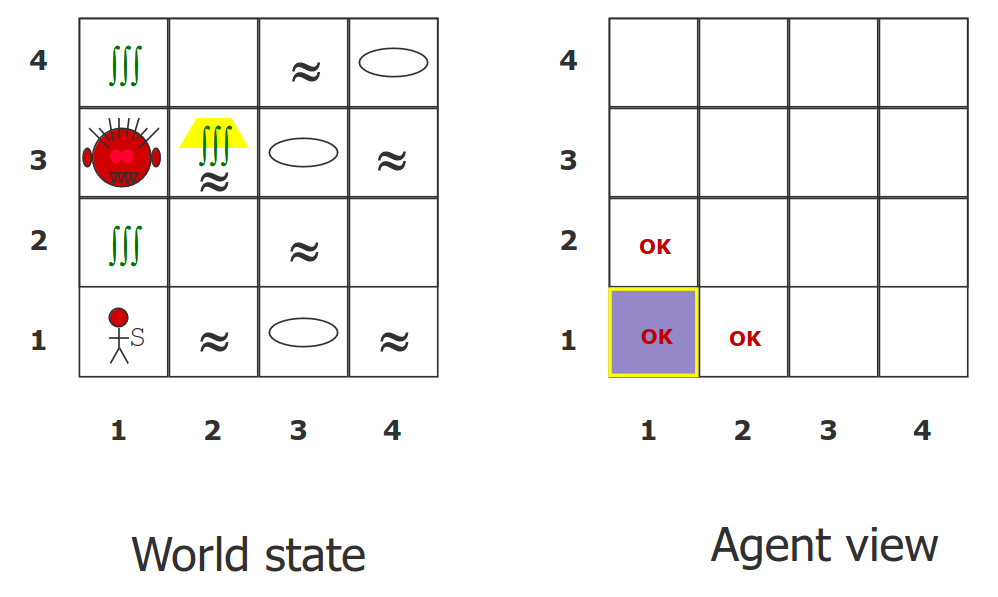
\includegraphics[width=0.8\textwidth]{img/wumpus.png}
		\end{figure}
		
		Avant de faire une action, l'agent dois "réfléchir" a propos de :
		\begin{itemize}
			\item analyser le state actuelle
			\item Eviter les dangers (wumpus et puits)
			\item Trouver le trésor
			\item Garder une version de l'environement (map, propirété des case ...)
		\end{itemize}
		
		\begin{figure}[H]
			\centering
			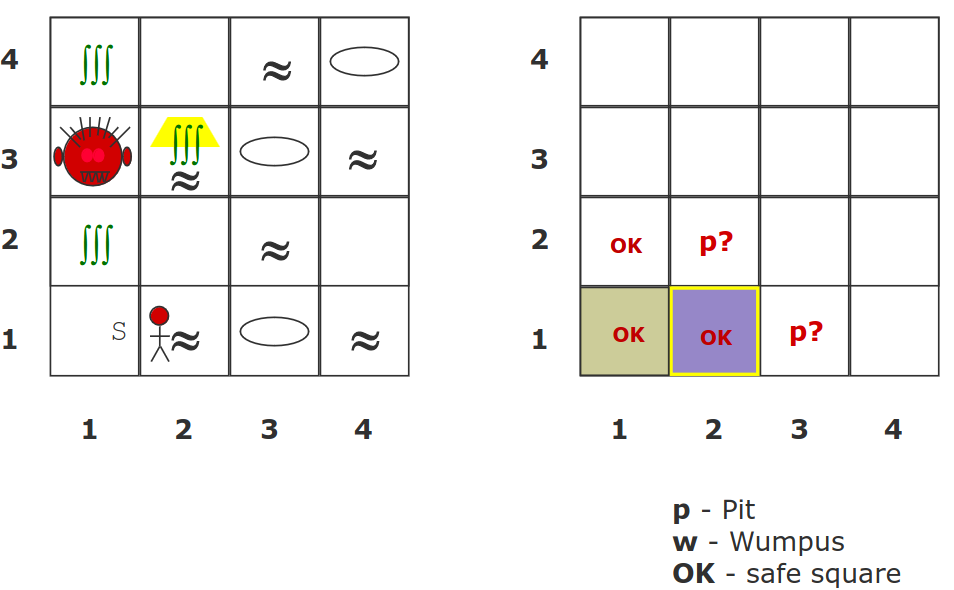
\includegraphics[width=0.8\textwidth]{img/wumpus1.png}
		\end{figure}
		
		\begin{figure}[H]
			\centering
			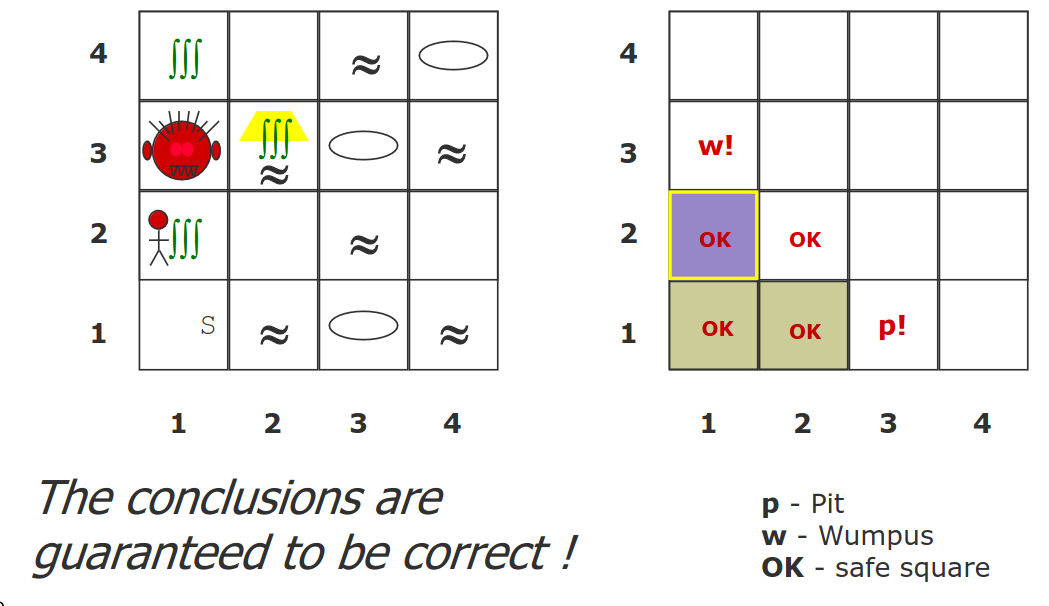
\includegraphics[width=0.8\textwidth]{img/wumpus2.png}
		\end{figure}
		
		\begin{figure}[H]
			\centering
			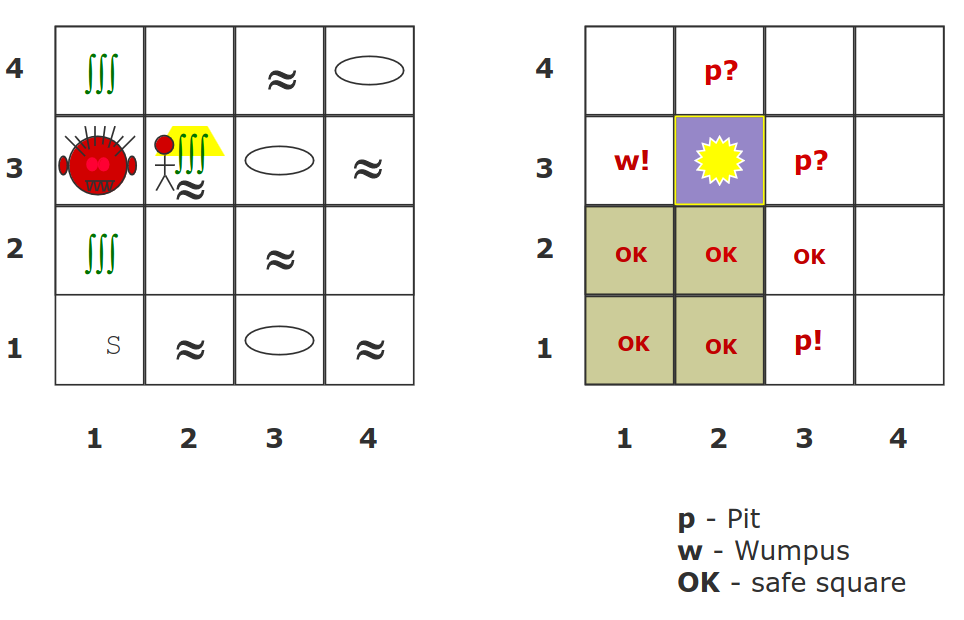
\includegraphics[width=0.8\textwidth]{img/wumpus3.png}
		\end{figure}
	\subsection{Logique}
		
		La logic correspond a de la syntax et de la sémantique
		\begin{itemize}
			\item \textbf{Syntax} : Spécifie toutes les phrases bien formé ($x+y=4$ OK $x2y+=$ KO)
			\item \textbf{Sémantique} : Définir la vérité des phrases par rapport à chaque monde possible
			\begin{itemize}
				\item $x=1, y=3$
				\item $x=2, y=2$
				\item \dots
			\end{itemize}
			\item \textbf{Interprétation} : abstraction mathématique d'un monde possible, en donnant une interprétation une phrase est vrai ou fausse.
			\item \textbf{Modele de phrase} : $\alpha$ est un interprétation ou la phrase est vraie.
			
			"\textit{$m$ est un model de $\alpha$}" $\rightarrow$ $\alpha$ est vrai dans l'interprétation de $m$
			\item \textbf{M($\alpha$)} : ensemble des modeles de $\alpha$
			\item KB $\models$ $\alpha$ : $\alpha$ est vrai si KB est vrai
			\item KB $\vdash$ $\alpha$ : On peut prouver $\alpha$ avec KB 

		\end{itemize}
		
	\subsubsection{Implication (entailment)}
		Implication entre la phrase $\alpha$ et $\beta$, $\beta$ est un conséquence logique de $\alpha$
		
		\begin{equation}
		\alpha \models \beta \ IFF \ M(\alpha) \subset M(\beta)
		\end{equation}
		
		$\beta$ est vrai dans chaque model de $\alpha$ (ex : $x=0 \models xy=0$)
		
		Dans le Wumpus game apres avoir rien détecter en [1,1] et bougé a droite et sentit la brize en [2,1] (signe d'un puit a coté de cette case).
		Toutes les interprétations possible pour KB en assumant seulement des pit est le suivant :
		
		\begin{figure}[H]
			\centering
			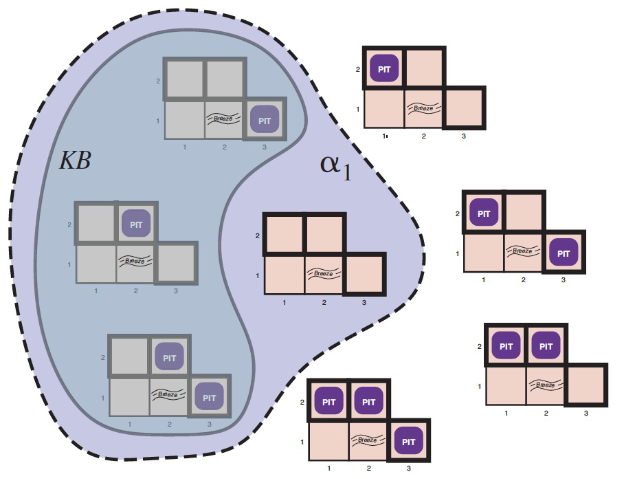
\includegraphics[width=0.8\textwidth]{img/modelsWumpus.png}
		\end{figure}
		
		\begin{itemize}
			\item KB = Regles de wumpus + observations
			\item $\alpha_1$ = "[1,2] est safe"
			\item KB $\models \alpha_1$, prouvé par models checking
		\end{itemize}
		
		\begin{figure}[H]
			\centering
			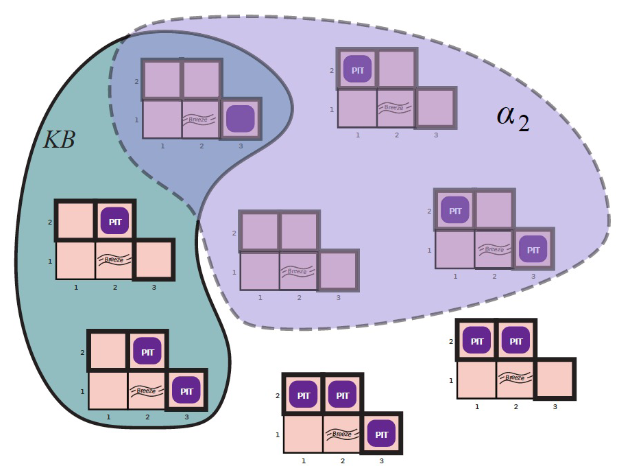
\includegraphics[width=0.8\textwidth]{img/modelsWumpus1.png}
		\end{figure}
		
		\begin{itemize}
			\item KB = Regles de wumpus + observations
			\item $\alpha_2$ = "[2,2] est safe"
			\item KB $\textcolor{red}{\not} \models \alpha_2$
		\end{itemize}
		
		
		si KB $\models$ $\alpha_1$ on peut conclure que $\alpha_1$ est vrai
		
		Verfier KB $\models$ $\alpha$ en utilisant le Model checking
		
		\begin{enumerate}
			\item énumération des interprétations
			\item Trouver les interprétations qui sont un models de $\alpha$
			\item Check que $\beta$ est vrai dans ces models $\alpha \vdash \beta$
		\end{enumerate}
		
		\begin{figure}[htp]	
			\centering
			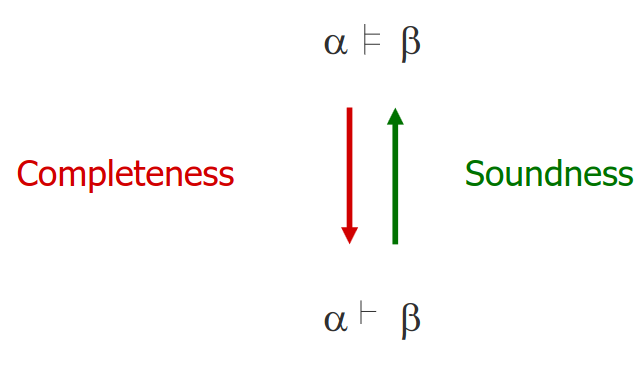
\includegraphics[width=0.4\textwidth]{img/KBA2.png}
		\end{figure}
		
		\subsubsection{Monotonicité}
			Si KB $\models \alpha$ alors KB $\land \beta \models \alpha$
			
			L'ensemble des formules empliqué ne peut que augmenterau fur et a mesure que des infos sont ajouter au KB
			
			Si une formule est impliquée par un sous ensemble de KB, il est alors aussi impliqué par KB
			
			\begin{figure}[htp]	
			\centering
			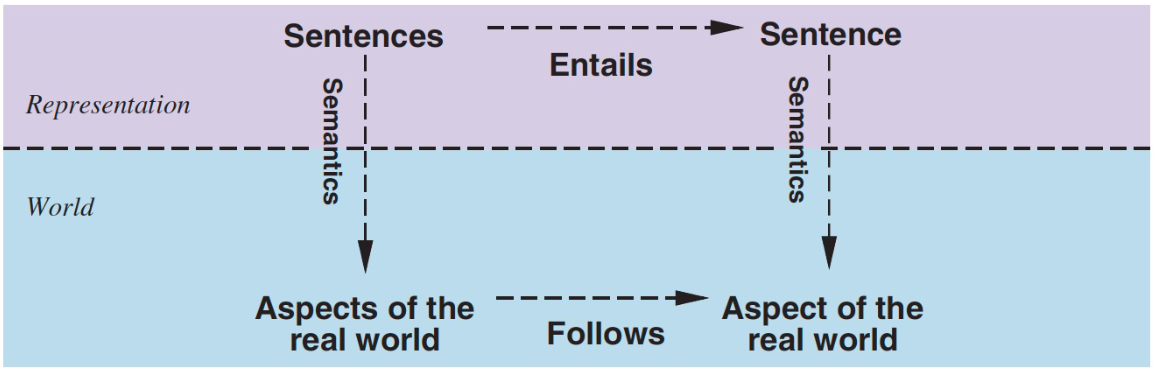
\includegraphics[width=\textwidth]{img/process.png}
		\end{figure}
		
	\subsection{Proposition logique}
		\subsubsection{Syntax}
			\begin{itemize}
				\item True, False
				\item Symbols (P,Q,A, \dots)
				\item Connecteur logiques :
				\begin{itemize}
					\item Négations : $\neg$
					\item Conjonctions : $\wedge$
					\item Disjonctions : $\vee$
					\item Implication : $\Rightarrow$
					\item Equivalence : $\Leftrightarrow$
					\item parenthese (,)
				\end{itemize}
			\end{itemize}
			
			\begin{figure}[htp]	
				\centering
				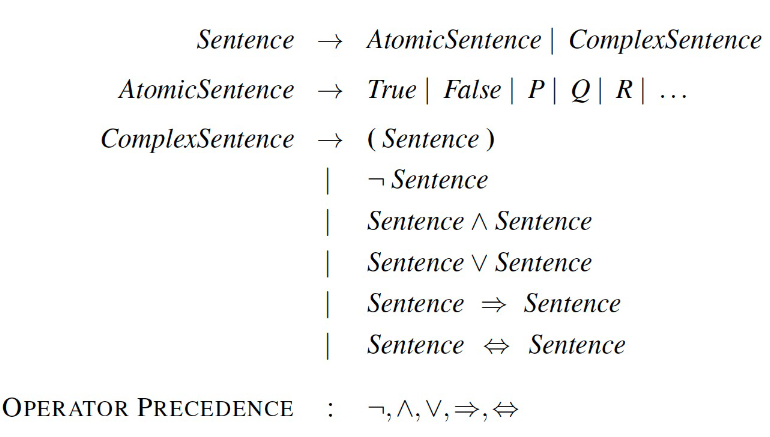
\includegraphics[width=0.6\textwidth]{img/KBA3.png}
			\end{figure}
			
			\subsubsection{Sémantique}
			On fait ça avec un table de verité
			\begin{figure}[H]	
				\centering
				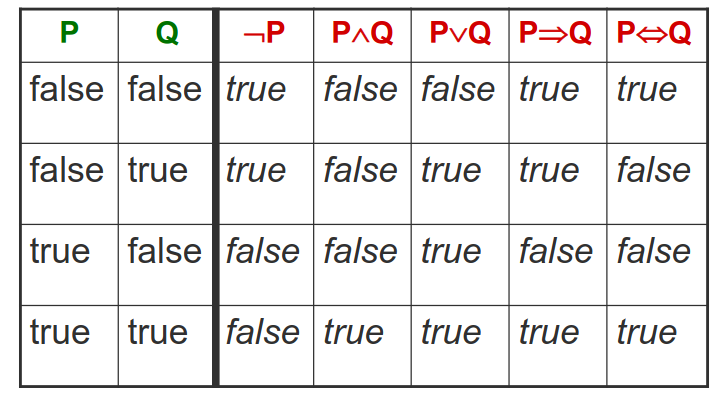
\includegraphics[width=0.6\textwidth]{img/KBA4.png}
			\end{figure}
			
			exemple Wumpus : Un carré est venteux si et seulement si un carré voisins est un puits
			
			$B_{1,1} \Leftrightarrow (P_{1,2} \vee P_{2,1})$
			
			\begin{figure}[htp]	
			\centering
			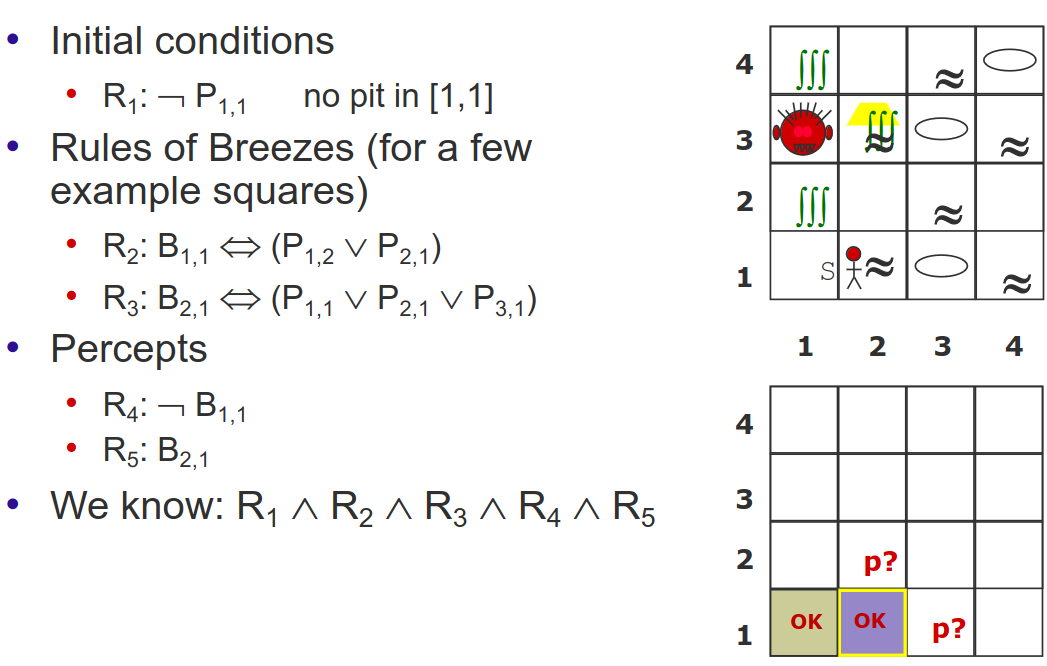
\includegraphics[width=0.8\textwidth]{img/KB.png}
		\end{figure}			
		\subsubsection{Inference}
			Le but est de decider si KB $\models \alpha$
			
			On veut savoir si $P_{1,2}$ n'est pas un puit :$\neg P_{1,2}$
			\begin{itemize}
				\item Imaginons nous avons ses infos : $B_{1,1}, B_{2,1}, P_{1,1}, P_{1,2}, P_{2,1}, P_{2,2}, P_{3,1}$
				\item on a donc $2^n$ interprétation possible ($n$ = nombre de symbol) donc ici $2^7$
			\end{itemize}
			
			Il faut donc enuméré sur chaque interprétation et check si $\alpha = P_{1,2}$ est True dans chaque models de KB
			
			Complexité temporelle de $\mathcal{O}(2^n)$ et spatiale de $\mathcal{O}(n)$
			
			\begin{figure}[htp]	
				\centering
				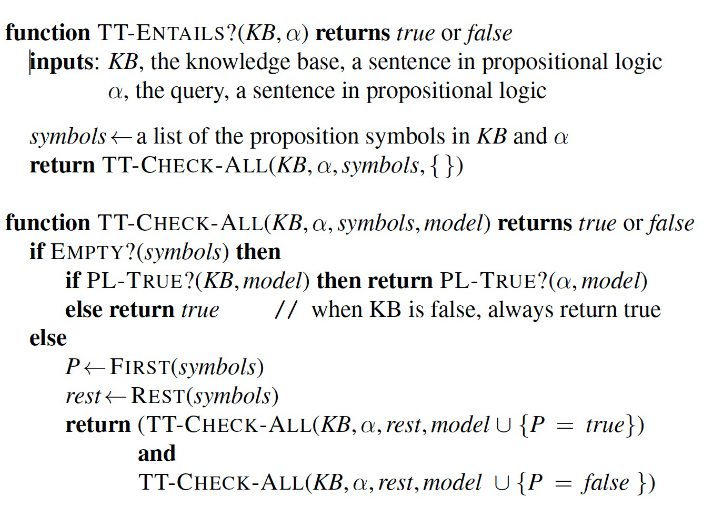
\includegraphics[width=0.6\textwidth]{img/KBA5.png}
			\end{figure}
			
	\subsection{Propositional Theorem Proving}
		\begin{itemize}
			\item Equivalence logique : $\alpha \equiv \beta$
			\item Valide (tautologie) : Toutes les intrerprétation sont valide (True)
			\item Satifaisant : True dans certaine interprétation mais pas toutes
			\item Unsatisfait : True pour aucune des interprétations.
			
		\end{itemize}
		
		$\alpha \models \beta IF (\alpha \wedge \neg\beta)$ est insatisfait
			
		\subsubsection{Preuve inference}
			\begin{itemize}
				\item Modus Ponens : $\cfrac{\alpha \Rightarrow \beta, \ \alpha}{\beta}$
				\item And-elimination : $\cfrac{\alpha \wedge \beta}{\alpha}$
				\item Two sens de Morgan : $\cfrac{\neg(\alpha\wedge\beta)}{\neg \alpha \vee \neg \beta} \Leftrightarrow \cfrac{\neg \alpha\vee\neg\beta}{\neg (\alpha \wedge\beta)}$

			\end{itemize}
			
		TODO A TERMINER
		